\documentclass[11pt]{article}
\usepackage[margin=2cm,headheight=14pt]{geometry}
\usepackage{amsmath,amssymb}
\usepackage{multicol}
\usepackage{tikz}
\usepackage{fancyhdr}

\pagestyle{fancy}
\fancyhf{}
\fancyhead[L]{Astroestadística}
\fancyhead[R]{Semestre 2026\text{-}2}
\renewcommand{\headrulewidth}{0.4pt}

\begin{document}
\section*{Quiz 2: aceptación y rechazo}

\textbf{Nombre:} \rule{7cm}{0.4pt}\hfill
\textbf{Puntaje:} \rule{1.5cm}{0.4pt} / 10

Cada pregunta vale 1 punto. Marque una sola opción por pregunta.

\begingroup
\setlength{\parskip}{0pt}
\begin{multicols}{2}
\raggedright{}
\begin{enumerate}
    \setlength{\itemsep}{0.7em}
    \item
    \begin{samepage}
    Si la propuesta es uniforme en $[0,1]$ con $q(x)=1$ y la función
    objetivo satisface $f(x)\leq 2$ en todo el intervalo, ¿cuál es una
    envolvente válida y su valor de $M$?
    \begin{enumerate}
        \item $h(x)=1$ y $M=1$.
        \item $h(x)=2$ y $M=2$.
        \item $h(x)=2(1-x)$ y $M=2$.
    \end{enumerate}

\end{samepage}

    \item
    \begin{samepage}
    Se propone $x=0.4$ y se obtiene $U=0.7$. Si
    $f(x)/(Mq(x))=0.6$, ¿qué decisión corresponde?
    \begin{enumerate}
        \item Se acepta porque $U<0.6$.
        \item Se acepta porque $x<0.5$.
        \item Se rechaza porque $U>0.6$.
    \end{enumerate}

\end{samepage}

    \item
    \begin{samepage}
    Si $f(x)=6x(1-x)$ en $[0,1]$ y se propone con $q(x)=1$, ¿cuál es
    el menor valor válido de $M$?
    \begin{enumerate}
        \item $M=1$.
        \item $M=3/2$.
        \item $M=3$.
    \end{enumerate}

\end{samepage}

    \item
    \begin{samepage}
    Si $f$ y $q$ son densidades normalizadas y se usa una envolvente con
    $M=3$, ¿cuál es la probabilidad total de aceptación?
    \begin{enumerate}
        \item $1/9$.
        \item $1/3$.
        \item $3/4$.
    \end{enumerate}

\end{samepage}

    \item
    \begin{samepage}
    Se generan $1000$ puntos uniformes en un rectángulo de área $8$ y
    $300$ caen bajo la curva. ¿Cuál es la estimación del área bajo la curva?
    \begin{enumerate}
        \item $0.3$.
        \item $2.4$.
        \item $8$.
    \end{enumerate}
\end{samepage}
\end{enumerate}
\end{multicols}
\endgroup

\newpage
\begingroup
\setlength{\parskip}{0pt}
\begin{multicols}{2}
\raggedright{}
\begin{enumerate}
    \setcounter{enumi}{5}
    \setlength{\itemsep}{0.7em}
    \item
    \begin{samepage}
    ¿Qué condición sobre la propuesta $q$ es necesaria para poder
    generar toda la distribución objetivo $f$?
    \begin{enumerate}
        \item $q(x)>0$ dondequiera que $f(x)>0$.
        \item $q(x)=f(x)$ para todo $x$.
        \item $q(x)=0$ dondequiera que $f(x)>0$.
    \end{enumerate}

\end{samepage}

    \item
    \begin{samepage}
    Si se aumenta $M$ aunque la envolvente siga siendo válida, ¿qué
    ocurre en general?
    \begin{enumerate}
        \item Aumenta la proporción aceptada.
        \item Disminuye la proporción aceptada.
        \item La proporción aceptada siempre permanece igual.
    \end{enumerate}

\end{samepage}

    \item
    \begin{samepage}
    ¿Qué papel cumple $U\sim\mathcal{U}(0,1)$ después de generar la
    propuesta $x$?
    \begin{enumerate}
        \item Determina si se conserva $x$, comparándolo con $f(x)/(Mq(x))$.
        \item Sustituye a la densidad propuesta $q(x)$.
        \item Se suma a $x$ para obtener la observación final.
    \end{enumerate}

\end{samepage}

    \item
    \begin{samepage}
    ¿Qué distribución siguen los valores que se aceptan?
    \begin{enumerate}
        \item La propuesta $q$ sin modificación.
        \item La distribución objetivo $f$.
        \item Una distribución uniforme en el soporte de $f$.
    \end{enumerate}
\end{samepage}
\end{enumerate}
\end{multicols}

\IfFileExists{Figuras/FigurasQuices/aceptacion_rechazo_quiz2.tex}
    {\input{Figuras/FigurasQuices/aceptacion_rechazo_quiz2.tex}}
    {\begin{center}
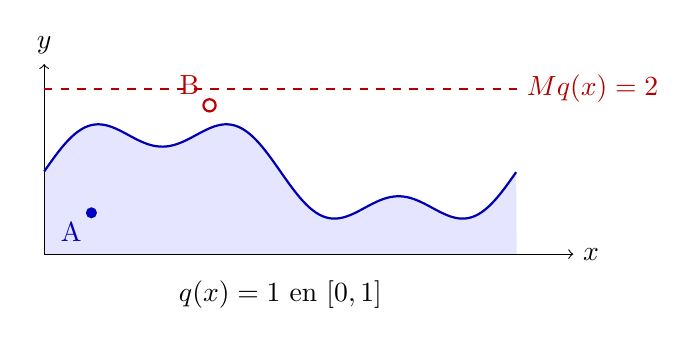
\begin{tikzpicture}[x=6cm,y=1.05cm]
  \fill[blue!10] (0,0) -- plot[domain=0:1,samples=140]
    (\x,{1+0.55*sin(360*\x)+0.25*sin(1080*\x)}) -- (1,0) -- cycle;
  \draw[->] (0,0) -- (1.12,0) node[right] {$x$};
  \draw[->] (0,0) -- (0,2.3) node[above] {$y$};
  \draw[thick,blue!70!black,domain=0:1,samples=140]
    plot (\x,{1+0.55*sin(360*\x)+0.25*sin(1080*\x)});
  \draw[thick,dashed,red!70!black] (0,2) -- (1,2)
    node[right] {$Mq(x)=2$};
  \fill[blue!75!black] (0.1,0.5) circle (2pt) node[below left] {A};
  \draw[red!75!black,thick] (0.35,1.8) circle (2.2pt)
    node[above left] {B};
  \node[below] at (0.5,-0.2) {$q(x)=1$ en $[0,1]$};
\end{tikzpicture}

\small La curva objetivo es $f(x)=1+0.55\sin(2\pi x)+0.25\sin(6\pi x)$.
\end{center}}
\begin{enumerate}
    \setcounter{enumi}{9}
    \setlength{\itemsep}{0.7em}
    \item
    \begin{samepage}
    La figura muestra puntos uniformes en el rectángulo bajo la
    envolvente $Mq(x)=2$. ¿Cuál afirmación interpreta correctamente
    tanto la probabilidad de aceptación en cada propuesta como el
    resultado para los puntos dibujados?
    \begin{enumerate}
        \item La probabilidad de aceptación es mayor en $x_A$ que en
        $x_B$; A se acepta y B se rechaza.
        \item La probabilidad de aceptación es mayor en $x_B$ que en
        $x_A$; A se acepta y B se rechaza.
        \item La probabilidad de aceptación es mayor en $x_A$ que en
        $x_B$; se aceptan ambos puntos.
    \end{enumerate}
\end{samepage}
\end{enumerate}
\endgroup

\end{document}